% questions.tex —— 2007 年·全国大纲卷Ⅱ·理科 · 题目内容片段（无答案）
% 由 tools/generate_projects.py 依来源总账自 2007/2007_数学真题_全国2理_试题.md 生成，勿手改（改源 MD 后重跑）


\gkpart{数学}

\begin{gktip}
\textbf{来源说明}：本题面依据固定源 PDF 两页 A3 题面逐题转录，原卷印刷页码 363–364。固定源不附答案，答案和解析均由本库独立复算；upstream 文件名按来源清单原样保留。

\textbf{图形说明}：第 19 题的原卷图形关系重绘为 TikZ/PGFPlots 矢量图。图形标记所指的 PNG 不随仓库保存。
\end{gktip}

\gkpart{一、选择题}

\begin{question}
\gkti{1}$\sin210^\circ=$\mbox{（　　）}

（A）$\dfrac{\sqrt3}{2}$\quad（B）$-\dfrac{\sqrt3}{2}$\quad（C）$\dfrac12$\quad（D）$-\dfrac12$

\end{question}
\begin{question}
\gkti{2}函数 $f(x)=|\sin x|$ 的一个单调递增区间是\mbox{（　　）}

（A）$\left(-\dfrac\pi4,\dfrac\pi4\right)$\quad（B）$\left(\dfrac\pi4,\dfrac{3\pi}4\right)$\quad（C）$\left(\pi,\dfrac{3\pi}2\right)$\quad（D）$\left(\dfrac{3\pi}2,2\pi\right)$

\end{question}
\begin{question}
\gkti{3}设复数 $z$ 满足 $\dfrac{1+2i}{z}=i$，则 $z=$\mbox{（　　）}

（A）$-2+i$\quad（B）$-2-i$\quad（C）$2-i$\quad（D）$2+i$

\end{question}
\begin{question}
\gkti{4}以下四个数中的最大者是\mbox{（　　）}

（A）$(\ln2)^2$\quad（B）$\ln(\ln2)$\quad（C）$\ln\sqrt2$\quad（D）$\ln2$

\end{question}
\begin{question}
\gkti{5}在 $\triangle ABC$ 中，已知 $D$ 是 $AB$ 边上一点，若 $\overrightarrow{AD}=2\overrightarrow{DB}$，$\overrightarrow{CD}=\dfrac13\overrightarrow{CA}+\lambda\overrightarrow{CB}$，则 $\lambda=$\mbox{（　　）}

（A）$\dfrac23$\quad（B）$\dfrac13$\quad（C）$-\dfrac13$\quad（D）$-\dfrac23$

\end{question}
\begin{question}
\gkti{6}不等式 $\dfrac{x-1}{x^2-4}>0$ 的解集为\mbox{（　　）}

（A）$(-2,1)$\quad（B）$(2,+\infty)$\quad（C）$(-2,1)\cup(2,+\infty)$\quad（D）$(-\infty,-2)\cup(1,+\infty)$

\end{question}
\begin{question}
\gkti{7}已知正三棱柱 $ABC-A_1B_1C_1$ 的侧棱长与底面边长相等，则 $AB_1$ 与侧面 $ACC_1A_1$ 所成角的正弦等于\mbox{（　　）}

（A）$\dfrac{\sqrt6}{4}$\quad（B）$\dfrac{\sqrt{10}}4$\quad（C）$\dfrac{\sqrt2}2$\quad（D）$\dfrac{\sqrt3}2$

\end{question}
\begin{question}
\gkti{8}已知曲线 $y=\dfrac{x^2}{4}-3\ln x$ 的一条切线的斜率为 $\dfrac12$，则切点的横坐标为\mbox{（　　）}

（A）$3$\quad（B）$2$\quad（C）$1$\quad（D）$\dfrac12$

\end{question}
\begin{question}
\gkti{9}把函数 $y=e^x$ 的图象按向量 $\boldsymbol a=(2,3)$ 平移，得到 $y=f(x)$ 的图象，则 $f(x)=$\mbox{（　　）}

（A）$e^{x-3}+2$\quad（B）$e^{x+3}-2$\quad（C）$e^{x-2}+3$\quad（D）$e^{x+2}-3$

\end{question}
\begin{question}
\gkti{10}从 $5$ 位同学中选派 $4$ 位同学在星期五、星期六、星期日参加公益活动，每人一天，要求星期五有 $2$ 人参加，星期六、星期日各有 $1$ 人参加，则不同的选派方法共有\mbox{（　　）}

（A）$40$ 种\quad（B）$60$ 种\quad（C）$100$ 种\quad（D）$120$ 种

\end{question}
\begin{question}
\gkti{11}设 $F_1,F_2$ 分别是双曲线 $\dfrac{x^2}{a^2}-\dfrac{y^2}{b^2}=1$ 的左、右焦点。若双曲线上存在点 $A$，使 $\angle F_1AF_2=90^\circ$，且 $|AF_1|=3|AF_2|$，则双曲线离心率为\mbox{（　　）}

（A）$\dfrac{\sqrt5}{2}$\quad（B）$\dfrac{\sqrt{10}}2$\quad（C）$\dfrac{\sqrt{15}}2$\quad（D）$\sqrt5$

\end{question}
\begin{question}
\gkti{12}设 $F$ 为抛物线 $y^2=4x$ 的焦点，$A,B,C$ 为该抛物线上三点。若 $\overrightarrow{FA}+\overrightarrow{FB}+\overrightarrow{FC}=0$，则 $|\overrightarrow{FA}|+|\overrightarrow{FB}|+|\overrightarrow{FC}|=$\mbox{（　　）}

（A）$9$\quad（B）$6$\quad（C）$4$\quad（D）$3$

\end{question}
\gkpart{二、填空题}

\begin{question}
\gkti{13}$(1+2x^2)\left(x-\dfrac1x\right)^8$ 的展开式中常数项为\gkblank{}。（用数字作答）

\end{question}
\begin{question}
\gkti{14}在某项测量中，测量结果 $\xi$ 服从正态分布 $N(1,\sigma^2)\ (\sigma>0)$。若 $\xi$ 在 $(0,1)$ 内取值的概率为 $0.4$，则 $\xi$ 在 $(0,2)$ 内取值的概率为\gkblank{}。

\end{question}
\begin{question}
\gkti{15}一个正四棱柱的各个顶点在一个直径为 $2\mathrm{cm}$ 的球面上。如果正四棱柱的底面边长为 $1\mathrm{cm}$，那么该棱柱的表面积为\gkblank{} $\mathrm{cm}^2$。

\end{question}
\begin{question}
\gkti{16}已知数列的通项 $a_n=-5n+2$，其前 $n$ 项和为 $S_n$，则 $\displaystyle\lim_{n\to\infty}\dfrac{S_n}{n^2}=$\gkblank{}。

\end{question}
\gkpart{三、解答题}

\begin{question}
\gkti{17}在 $\triangle ABC$ 中，已知内角 $A=\dfrac\pi3$，边 $BC=2\sqrt3$，设内角 $B=x$，周长为 $y$。

（1） 求函数 $y=f(x)$ 的解析式和定义域；

（2） 求 $y$ 的最大值。

\end{question}
\begin{question}
\gkti{18}从某批产品中，有放回地抽取产品二次，每次随机抽取 $1$ 件，假设事件 $A$：“取出的 $2$ 件产品中至多有 $1$ 件是二等品”的概率 $P(A)=0.96$。

（1） 求从该批产品中任取 $1$ 件是二等品的概率 $p$；

（2） 若该批产品共有 $100$ 件，从中任意抽取 $2$ 件，$\xi$ 表示取出的 $2$ 件产品中二等品的件数，求 $\xi$ 的分布列。

\Needspace{0.4\textheight}
\end{question}
\begin{question}
\gkti{19}如图，在四棱锥 $S-ABCD$ 中，底面 $ABCD$ 为正方形，侧棱 $SD\perp$ 底面 $ABCD$，$E\text{、}F$ 分别是 $AB\text{、}SC$ 的中点。
\nopagebreak[4]
\begin{center}% 2007 年全国大纲卷Ⅱ理科第 19 题：正方形底面四棱锥
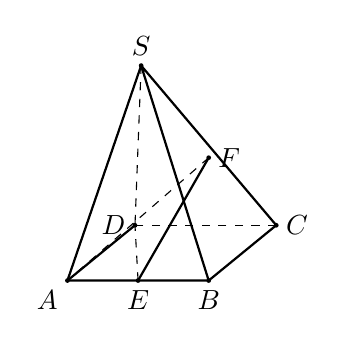
\begin{tikzpicture}[>=stealth,scale=0.78]
  \coordinate (A) at (0,0); \coordinate (B) at (2.3,0);
  \coordinate (C) at (3.4,0.9); \coordinate (D) at (1.1,0.9);
  \coordinate (S) at (1.2,3.5); \coordinate (E) at (1.15,0);
  \coordinate (F) at (2.3,2.0);
  \draw[thick] (A)--(B)--(C); \draw[dashed] (C)--(D); \draw[thick] (D)--(A);
  \draw[thick] (S)--(A) (S)--(B) (S)--(C);
  \draw[dashed] (S)--(D);
  \draw[thick] (E)--(F);
  \draw[dashed] (E)--(D) (F)--(A);
  \fill (S) circle (1.1pt) node[above] {$S$};
  \fill (A) circle (1.1pt) node[below left] {$A$};
  \fill (B) circle (1.1pt) node[below] {$B$};
  \fill (C) circle (1.1pt) node[right] {$C$};
  \fill (D) circle (1.1pt) node[left] {$D$};
  \fill (E) circle (1.1pt) node[below] {$E$};
  \fill (F) circle (1.1pt) node[right] {$F$};
\end{tikzpicture}
\end{center}
\nopagebreak[4]
（1） 求证：$EF\parallel$ 平面 $SAD$；

（2） 设 $SD=2CD$，求二面角 $A-EF-D$ 的大小。

\end{question}
\begin{question}
\gkti{20}在直角坐标系 $xOy$ 中，以 $O$ 为圆心的圆与直线 $x-\sqrt3y=4$ 相切。

（1） 求圆 $O$ 的方程；

（2） 圆 $O$ 与 $x$ 轴相交于 $A,B$ 两点，圆内的动点 $P$ 使 $|PA|,|PO|,|PB|$ 成等比数列，求 $\overrightarrow{PA}\cdot\overrightarrow{PB}$ 的取值范围。

\end{question}
\begin{question}
\gkti{21}设数列 $\{a_n\}$ 的首项 $a_1\in(0,1)$，$a_n=\dfrac{3-a_{n-1}}2$，$n=2,3,4,\ldots$。

（1） 求 $\{a_n\}$ 的通项公式；

（2） 设 $b_n=a_n\sqrt{3-2a_n}$，证明 $b_n<b_{n+1}$，其中 $n$ 为正整数。

\end{question}
\begin{question}
\gkti{22}已知函数 $f(x)=x^3-x$。

（1） 求曲线 $y=f(x)$ 在点 $M(t,f(t))$ 处的切线方程；

（2） 设 $a>0$，如果过点 $(a,b)$ 可作曲线 $y=f(x)$ 的三条切线，证明：$-a<b<f(a)$。

\end{question}